\documentclass[12pt]{article}
\usepackage{hyperref}
\usepackage{graphicx}
\usepackage[font=small,labelfont=bf]{caption}
\title{Progetto di fine corso}
\date{05/09/2016}
\author{Alessio Luca,Carlo Sindico}

\begin{document}
	\pagenumbering{arabic}
	
	\begin{titlepage}
		\newcommand{\HRule}{\rule{\linewidth}{0.5mm}}%linea orizzontale
		\center
		
		\textsc{\LARGE Universit\`a degli Studi di Padova}\\[1.5cm] 
		\textsc{\Large Laurea in Informatica}\\[0.5cm]
		\textsc{\large Corso di Tecnologie Web}\\[0.5cm]
		\textsc{\large Progetto di fine corso}\\[0.5cm]
		
		%----------------------------------------------------------------------------------------
		%	TITLE SECTION
		%----------------------------------------------------------------------------------------
		
		\HRule \\[0.4cm]
		{ \huge  Parco Naturale Monte Verde}\\[0.3cm] 
		\HRule \\[0.4cm]
		
		
		%----------------------------------------------------------------------------------------
		%	AUTHOR SECTION
		%----------------------------------------------------------------------------------------
		
		\begin{minipage}{0.3\textwidth}
			\begin{flushleft} \large
				\emph{Studente:}\\
				Luca \textsc{Alessio} % Your name
			\end{flushleft}
		\end{minipage}
		~
		\begin{minipage}{0.3\textwidth}
			\begin{flushright} \large
				\emph{Matricola:} \\
				\textsc{1070690} % Supervisor's Name
			\end{flushright}
		\end{minipage}\\[1cm]
		
			\begin{minipage}{0.3\textwidth}
				\begin{flushleft} \large
					\emph{Studente:}\\
					Carlo \textsc{Sindico} % Your name
				\end{flushleft}
			\end{minipage}
			~
			\begin{minipage}{0.3\textwidth}
				\begin{flushright} \large
					\emph{Matricola:} \\
					\textsc{1069322} % Supervisor's Name
				\end{flushright}
			\end{minipage}\\[1cm]
			
		%----------------------------------------------------------------------------------------
		%	INFORMATION WEBSITE
		%----------------------------------------------------------------------------------------
		
		\textsc{\Large Link al sito:}\\[0.2cm]	
		\textit{//tecnologie-web.studenti.math.unipd.it/tecweb/$\sim$csindico/}\\[1cm]
		
		\textsc{\Large Mail del referente:}\\[0.2cm]	
		\textit{sindycarlo@gmail.com}\\[1cm]
		
		%----------------------------------------------------------------------------------------
		%	DATI LOGIN
		%----------------------------------------------------------------------------------------
		
			\textsc{\Large Login Admin:}\\[0.2cm]
			\textsc{ Username:}\textit{ admin }\\[0.1mm]
			\textsc{ Password:}\textit{ admin }\\[0.1mm]
			
		\vfill
	\end{titlepage}
	
	\newpage
	\renewcommand{\contentsname}{Indice}
	\tableofcontents
	
	
	\newpage
	\pagenumbering{arabic}
	
	\section{Abstract}
	\begin{itemize}
		\item Il sito realizzato riguarda il fittizio Parco Naturale Monte Verde.\\ L'obiettivo principale che il portale monteverde.it si pone \`e quello di fornire tutte le informazioni possibili sul parco agli utenti visitatori. Il sito \`e in lingua italiana.
		
		\item L'utenza che accede al sito ha la possibilit\`a di visualizzare pagine informative che descrivono flora, fauna, storia e conformazione del parco e le attivit\`a che si possono svolgere al suo interno.

		\item Nel sito sono presenti anche pagine contenenti contenuto dinamico come gli orari e i prezzi d'ingresso al parco ed una pagina dedicata alle notizie.

		\item L'amministratore del sito ha la possibilit\`a di alterare prezzi ed orari del parco e di creare nuove notizie.\\ \\ Una dettagliata spiegazione sulle funzionalit\`a accessibili dall'amministratore \`e presente nella sezione "Amministrazione del sito".

		\item \textbf{Disclaimer:} Il Parco Naturale Monte Verde \`e un luogo puramente fantastico e senza alcuna corrispondenza nel mondo reale.\\ \\ La maggior parte dei testi contenuti nel nostro sito sono stati presi in prestito da http://www.pnab.it/ perch\`e, nonostante il Parco Naturale Monte Verde sia un luogo fittizio, ci \`e sembrato poco elegante riempire le pagine di "lorem ipsum" e allo stesso tempo la stesura di testo verosimile e originale avrebbe richiesto troppo tempo.\\ \\ Per quanto riguarda le immagini, esse sono state ricercate tramite Google Images, su richiesta del docente possiamo fornire la provenienza di ciascuna immagine (non includeremo tali dati in questa relazione in quanto superflui).\\ \\ Il logo \`e stato preso dal sito https://greenmountainbaptist.org/ .

	\end{itemize}

\newpage

\section{Materiale consegnato}
			
			 I file consegnati sono organizzati su quattro cartelle:
			\begin{itemize}
				\item cgi-bin: cartella nella quale sono presenti i file .cgi
				\item data: in questa cartella sono contenuti i file .xml ed i relativi .xsd
				\item public-html: contiene i file .html e le sotto-cartelle:
\begin{itemize}
\item css: cartella contenente i file .css
		\item		 images: cartella contenente tutte le foto del sito
			\item	 js: cartella contenente i vari script realizzati in JavaScript
\end{itemize}		
\item relazione: cartella contenente la presente relazione in formato .pdf e le immagini in essa contenute a dimensioni originali		 
			\end{itemize}	
			Ciascun file verr\`a esaminato in dettaglio nelle successive sezioni. 
			
			\newpage

\section{Struttura del sito}
Il sito \`e diviso nelle seguenti aree primarie: 
		\begin{itemize}
			\item \textbf{Home}: pagina di benvenuto, contiene una breve descrizione del parco e vari link alle sezioni principali del sito
			\item \textbf{Chi Siamo}: pagina puramente a scopo informativo, contiene un elenco degli avvenimenti importanti nella storia del parco, dall'inaugurazione al giorno d'oggi
			\item \textbf{Natura e Territorio}: altra pagina descrittiva, fornisce informazioni sulla conformazione territoriale del parco e su flora e fauna presenti in esso
			\item \textbf{News e Attivit\`a}: pagina divisa in due sezioni, un primo settore riguardante le attivit\`a che \`e possibile svolgere nel parco ed una seconda zona contente le notizie pi\`u recenti
			\item \textbf{Orari e Prezzi}: come suggerisce il nome, da questa pagina l'utente pu\`o conoscere orari e prezzi d'ingresso al parco
			\item \textbf{Info e Contatti}: contiene informazioni quali il regolamento del parco, le istruzioni per raggiungerlo e contatti utili
		\end{itemize}				
Da ogni pagina \`e possibile raggiungere la Mappa del Sito dal link posto prima del footer.	

\newpage

\section{Struttura delle pagine}
Le pagine del sito differiscono per contenuto ma condividono i seguenti elementi:
\begin{itemize}
\item \textbf{Header}: la parte superiore di ogni pagina contiene il logo (che linka alla home) e il nome del sito in alto a sinistra, subito sotto sono invece presenti dei collegamenti alle aree principali del sito (vedi Struttura del sito). L'header pu\`o essere saltato da un utente che utilizza uno screen reader tramite apposite ancore d'aiuto (vedi sezione Accessibilit\`a)
\item \textbf{Breadcrumb}: rende noto all'utente la sua posizione precisa all'interno del sito, dal breadcrumb \`e possibile risalire alle pagine precedentemente visitate
\item \textbf{Link d'aiuto}: in ogni pagina \`e sempre presente un link alla Mappa del Sito e l'ancora "Torna all'Inizio" che riporta la visuale all'inizio della pagina, utile nelle pagine con contenuto corposo
\item \textbf{Footer}: contiene brevi informazioni come l'indirizzo del parco e le certificazioni di aderenza agli standard del sito; dal footer \`e possibile loggare/sloggare come amministratore
\end{itemize}

\newpage

\section{Amministrazione del sito}
\textit{Login:} admin \textit{Password:} admin
\begin{itemize}
\item \`E possibile accedere all'area amministrativa da qualsiasi pagina tramite un link posto nel footer.
\item L'amministratore ha la possibilit\`a di modificare gli orari e i prezzi d'ingresso al parco utilizzando i form appositi. 
\item I form presentano delle liste a cascata da cui \`e possibile scegliere il preciso dato da modificare (una lista con i giorni della settimana per gli orari, due liste con tipologia e periodo di validit\`a per il prezzo del biglietto) e un campo testuale in cui inserire i nuovi valori.\\ \\ Il form per il cambio dell'orario accetta qualsiasi input testuale (perch\`e sono permessi sia valori misti come "8:30 - 18:30" sia valori puramente testuali come "Chiuso") mentre il prezzo del biglietto dovr\`a necessariamente essere un intero.
\item L'amministratore pu\`o pubblicare nuove notizie riguardanti eventi, promozioni e attivit\`a inerenti al parco. Di una notizia \`e necessario conoscere il titolo, il corpo dell'articolo e un' immagine ad essa associata (oltre alla data che per\`o viene automaticamente memorizzata dal sistema senza dover essere inserita manualmente).
\item L'amministratore pu\`o eliminare individualmente le varie notizie recandosi nella pagina "Archivio News" (News e Attivit\`a $\rightarrow$ Archivio News link in basso) e cliccando su "Elimina". Alternativamente \`e possibile eliminare una notizia direttamente nella pagina che la visualizza.
\item Quando l'amministratore \`e loggato il footer cambia (vedi footer\_manager.js) permettendo il logout tramite l'apposito pulsante o il ritorno all'area amministratore in caso ci si trovi in un'altra pagina.
\end{itemize}

\newpage

			\section{HTML}

Le pagine .html del sito sono state realizzate rispettando lo standard XHTML 1.0 Strict.\\ \\
Analizziamo brevemente il contenuto di ciascun file .html:
\begin{itemize}
\item \textit{index.html}: homepage del sito, contiene una breve descrizione del parco e vari link alle sezioni principali del sito
\item \textit{chisiamo.html}:  pagina puramente a scopo informativo, contiene un elenco degli avvenimenti importanti nella storia del parco, dall'inaugurazione al giorno d'oggi
\item \textit{naturaterritorio.html}:  altra pagina descrittiva, fornisce informazioni sulla conformazione territoriale del parco e su flora e fauna presenti in esso
\item \textit{flora.html}: altra pagina puramente informativa, accessibile passando da naturaterritorio.html, contiene una descrizione più approfondita della flora del parco
\item \textit{fauna.html}: altra pagina puramente informativa, accessibile passando da naturaterritorio.html, contiene una descrizione più approfondita della fauna del parco
\item \textit{infocontatti.html}: contiene informazioni quali il regolamento del parco, le istruzioni per raggiungerlo e contatti utili
\item \textit{regolamento.html}: accessibile da infocontatti.html, contiene una lista dei dieci punti da rispettare per rendere la propria permanenza al parco piacevole a se stessi e agli altri\\ (http://www.pnab.it/vivere-il-parco/10-regole-per-rispettare-il-parco.html)
\item \textit{attivita.html}: pagina di approfondimento sulle attività che si possono svolgere al Parco Naturale Monte Verde, è accessibile passando per newsattivita.cgi
\item \textit{mappasito.html}: mappa del sito, contiene collegamenti a tutte le zone principali e secondarie del sito
\end{itemize}
Si veda la sezione Javascript per ulteriori approfondimenti sulla generazione dinamica del footer.\\
Il codice .html rispetta interamente le imposizioni del validatore W3C https://validator.w3.org/ .

			\section{Perl} dire che alcune parti di codice sono ispirate dal vecchio progetto (semplici operazioni creazione eliminazione)
		
				  Le pagine scritte in Perl si dividono principalmente in due tipologie: pagine "dinamiche" di rappresentazione e pagine di elaborazione dei dati.\\ \\
				Alla prima tipologia appartengono i file .cgi che eseguono il "print" della pagina con il contenuto richiesto (ne \`e un esempio la pagina notizia.cgi che si occupa della stampa a video di una notizia) mentre le pagine della seconda tipologia sono solitamente "pagine di servizio" ovvero codice che esegue operazioni dietro le quinte come salvataggi ed eliminazioni di dati sui file xml. \\ \\Nel dettaglio, questo \`e ci\`o di cui ciascun file si occupa:
\begin{itemize}
\item \textit{adminlogin.cgi}: contiene il form che l'amministratore utilizza per effettuare l'accesso all'area riservata (vedi Cookies per Login e Logout)
\item \textit{controllologin.cgi}: controlla la correttezza delle credenziali inserite nel form della pagina adminlogin.cgi, se sono corrette reindirizza ad adminarea.cgi (in particolare verifica la correttezza dei valori dei cookie) altrimenti visualizza un messaggio d'errore (vedi Cookies per Login e Logout)
\item \textit{adminarea.cgi}: cuore dell'area amministrativa, da questa pagina l'admin ha la possibilit\`a di modificare orari e prezzi e di creare nuove notizie tramite gli appositi form
\item \textit{change\_orario.cgi}: si occupa di processare l'operazione di modifica di un orario e ne notifica l'esito all'amministratore visualizzando un messaggio positivo o negativo; viene richiamato in seguito all'invio dei dati del form per la modifica di un orario in adminarea.cgi
\item \textit{change\_prezzo.cgi}: si occupa di processare l'operazione di modifica di un prezzo e ne notifica l'esito all'amministratore visualizzando un messaggio positivo o negativo; viene richiamato in seguito all'invio dei dati del form per la modifica di un prezzo in adminarea.cgi
\item \textit{nuova\_notizia.cgi}: si occupa di processare l'operazione di creazione di una notizia e ne notifica l'esito all'amministratore visualizzando un messaggio positivo o negativo; viene richiamato in seguito all'invio dei dati del form per la creazione di una notizia in adminarea.cgi
\item \textit{delete\_notizia.cgi}: si occupa di processare l'operazione di eliminazione di una notizia e ne notifica l'esito all'amministratore visualizzando un messaggio positivo o negativo; viene richiamato in seguito alla pressione del tasto "Elimina" accanto a una notizia
\item \textit{logout.cgi}: codice richiamato alla pressione del tasto "Logout", effettua la disconnessione dell'account dell'amministratore (vedi Cookies per Login e Logout)
\item \textit{newsattivita.cgi}:  pagina divisa in due sezioni, un primo settore riguardante le attivit\`a che \`e possibile svolgere nel parco (sezione approfondita in attivita.html) ed una seconda zona contente le anteprime delle tre notizie pubblicate pi\`u di recente, da questa pagina \`e possibile accedere l'Archivio delle News (news.cgi) mediante il collegamento apposito posto di seguito alle notizie pi\`u recenti
\item \textit{news.cgi}: Archivio News, contiene un' anteprima di tutte le notizie presenti nel database ordinate cronologicamente dalla pi\`u recente: le notizie vengono visualizzate 4 alla volta per non deformare la pagina (e rendere i tempi di caricamento interminabili) qualora siano presenti un elevato numero di notizie, per caricare le notizie successive \`e sufficiente cliccare sul link "Carica altre notizie"; questa pagina riceve in ingresso un parametro tramite get, \`e semplicemente un indice per tenere traccia di dove si \`e arrivati nello scorrimento delle notizie nell .xml, in questo documento non esamineremo in dettaglio il suo utilizzo ma siamo pronti a fornire eventuali chiarimenti qualora il codice risulti poco chiaro; l'amministratore ha la possibilit\`a di eliminare una notizia tramite il tasto "Elimina"
\item \textit{notizia.cgi}: pagina a contenuto dinamico che visualizza una notizia completa, la pagina prende in input tramite get un parametro numerico corrispondente all'identificativo (ID nell' .xml) della notizia da visualizzare; l'amministratore ha la possibilit\`a di eliminare la notizia tramite il tasto "Elimina"
\item \textit{orarieprezzi.cgi}: pagina a contenuto dinamico che visualizza prezzi ed orari del parco
\item \textit{funzioni.pl}: contiene funzioni di servizio usate da diversi file .cgi
\end{itemize}	

\textbf{Disclaimer:} per quanto riguarda i file change\_orario.cgi, change\_prezzo.cgi, notizia.cgi, nuova\_notizia.cgi e delete\_notizia.cgi, essi sono stati riadattati da alcuni file dello scorso progetto. 
\\ Il motivo di tale riuso (sebbene parziale) \`e che le operazioni eseguite da tali file sono semplici passaggi basilari di lettura e scrittura/modifica su file .xml, ci sembrava perci\`o difficile e inutile riscrivere un codice che non fosse troppo analogo al precedente senza renderlo inutilmente pi\`u complicato; abbiamo preferito essere trasparenti comunicandole questa nostra scelta.\\ Il codice .html stampato dai file .cgi rispetta le imposizioni del validatore W3C https://validator.w3.org/ .

\subsection*{Cookies per Login e Logout}
Alcune osservazioni sulla procedura di accesso e uscita dall'account amministratore:
\begin{itemize}
\item \`E possibile accedere all'area riservata da ogni pagina tramite il link sul footer
\item Al primo accesso dell'amministratore nel sistema (ci troviamo quindi in adminlogin.cgi, le credenziali sono state inserite e il file controllologin.cgi le verifica) viene creato il cookie \textit{autorizzazione} se l'operazione di login avviene con successo.
\item Se un utente esterno prova ad accedere ad adminarea.cgi cambiando l'url nella barra degli indirizzi esso verr\`a intercettato da controllologin.cgi e reindirizzato ad una pagina di errore
\item Se l'admin prova ad accedere nuovamente al form per il login nonostante sia gi\`a loggato, controllologin.cgi lo reindirizza ad adminarea.cgi
\item \`E possibile ritornare in adminarea.cgi da ogni pagina tramite il link sul footer
\item \`E possibile sloggarsi da ogni pagina tramite il tasto "Logout" sul footer
\item Conoscendo il valore del cookie \textit{autorizzazione} \`e possibile stampare correttamente il footer (in versione login o logout)
\item logout.cgi molto semplicemente imposta il cookie \textit{autorizzazione} con un valore non accettato dal sistema
\end{itemize}
	
		\newpage	
	\section{CSS}
	\begin{itemize}
	
	
		\item Nella realizzazione dell'interfaccia grafica del sito \`e stato rispettato lo standard CSS3.
		\item Per il design del sito sono state adottate delle scelte il pi\`u possibile minimali per mantenere alti livelli di usabilit\`a
		\item Nella cartella \textit{public\_html/css/} sono presenti i seguenti fogli di stile:
		\begin{itemize}

				\item \textit{style.css:} modella lo stile di visualizzazione del sito sia per gli utenti desktop che per gli utenti che utilizzano tablet e dispositivi mobile

				\item \textit{styleprint.css:} regola la trasposizione su carta stampata del sito
		\end{itemize}
\item Per la realizzazione dell'header abbiamo preso spunto dalle direttive sull'accessibilit\`a messe a disposizione dal sito http://lau.csi.it/
\item Sono stati utilizzati fogli di stile CSS tali da rendere fruibile il contenuto delle pagine anche qualora essi fossero disabilitati o non supportati
\item I punti di rottura delle media query avvengono a 1350px, 922px e 769px per garantire una corretta visualizzazione su diverse risoluzioni
\item Si \`e prestata particolare attenzione al layout della homepage dove (in modalit\`a desktop) le categoria principali sono presenti nell'inquadratura principale evitando all'utente lo scroll del mouse
\item Il men\`u di navigazione posto nell'header \`e responsive e diventa verticale in versione smartphone
\item Il codice CSS rispetta le indicazioni del validatore W3C https://jigsaw.w3.org/css-validator/
		\end{itemize}
					\newpage
				
		\section{XML}
	Nella cartella \textit{data} sono presenti 4 file .xml principali con i rispettivi .xsd:

		\begin{itemize}
		\item \textit{newsparco}: funge da "database" del sito, ogni notizia presenta i seguenti campi di tipo stringa:
		\begin{itemize}
		\item titolo: titolo dell'articolo
		\item contenuto: contenuto dell'articolo
		\item data: data di creazione della notizia (salvata automaticamente)
		\item img: contiene l'url dell'immagine (le immagini sono salvate in \textit{public\_html/images/} ).
		Ogni notizia contiene inoltre l'attributo ID che funge da identificativo univoco.
		\end{itemize}
		\item \textit{orari}: contiene gli orari del parco, il tag principale orari contiene diversi tag giorno contraddistinti da un id (stringa contente il giorno della settimana) e contenenti un campo ora.\\
		Il campo ora \`e di tipo stringa perch\`e pu\`o contenere sia valori come "09:00-18:00" sia valori come "Chiuso".
		\item \textit{prezzi}: contiene i prezzi del parco, contiene tre tag \textit{ingresso} per le tre tipologie di biglietto (intero, ridotto ragazzi e ridotto anziani usati come id) ciascuno contente a sua volta due sottotag \textit{primaveraautunno} ed \textit{estate} per suddividere i prezzi in base al periodo dell'anno.
		\item  \textit{amministratore} semplice schema ausiliario per il controllo del corretto login nell'area amministrativa, contiene solamente due campi per il login e la password.
		\end{itemize}	
		I file .xml e i .xsd corrispondenti sono considerati validi dal validatore W3C http://www.utilities-online.info/xsdvalidation .			
					\newpage
			\section{Javascript}
				 Javascript \'e stato utilizzato principalmente per il controllo degli input nei form e per la generazione automatica del footer nelle pagine .html\\
				 Nel sito sono presenti 4 differenti form, quello per il login nell'area amministrativa ed i 3 form interni all'area amministrativa. \\
				 Analizziamo ora ciascun file .js presente nella cartella \textit{public\_html/js/}:
				 \begin{itemize}
				 \item \textit{amministratore.js}: gestisce il form di login segnalando eventuali campi mancanti
				 \item \textit{form.js}: gestisce il form per la modifica di un prezzo segnalando eventuali campi mancanti
				 \item \textit{form2.js}: gestisce il form per la modifica di un orario segnalando eventuali campi mancanti
				 \item \textit{form3.js}: gestisce il form per la creazione di una notizia segnalando eventuali campi mancanti
				 \item \textit{footer\_manager.js}: si occupa della generazione dinamica del footer nelle pagine .html:
				 \begin{itemize}
				 \item lo script viene eseguito al momento del caricamento della pagina grazie all'attributo \textit{onload} applicato al body
				 \item lo script analizza il valore attuale del cookie \textit{autorizzazione} (vedi Cookies per Login e Logout)
				 \item in base al valore del cookie viene aggiornato un innerHTML nel footer con l'elemento apposito
				 \end{itemize}
				 L'idea di usare l'attributo \textit{onload} \`e stata ispirata da alcune discussioni sul sito www.stackoverflow.com
				 \end{itemize}
				
	\newpage
		\section{Accessibilit\`a}
		\begin{itemize}
			\item Per semplificare l'utilizzo del sito e renderlo fruibile anche ad utenti diversamente abili si \'e optato per la separazione della struttura dalla presentazione e dal comportamento.
			\item Il contenuto del sito \'e  infatti racchiuso nei file .html e .cgi i quali richiamano fogli di stile .css, utilizzano script .js e interagiscono con file .xml per la lettura e la scrittura di dati.
			\item La compilazione dei form rimane sempre accessibile, opportuni controlli in Perl verificano comunque la validit\`a degli input emessi dall'utente anche se JavaScript \'e disabilitato.

			\item Tutto il codice \'e stato scritto seguendo le disposizioni W3C con opportuna validazione sui loro validatori.
		
				\item Si \'e scelto uno schema di colori non particolarmente vivace: essendo un sito che descrive un parco naturale, i colori scelti (verde chiaro e bianco) si avvicinano il pi\'u possibile al contenuto.

				\item I link sono sempre sottolineati e di colore blu (tranne nell'header), diventano di colore viola quando vengono visitati.
				\item In particolare nell'header, il link della pagina in cui si trova l'utente \'e di colore rosso per distinguerlo dagli altri link che possono essere di colore viola se sono gi\'a stati visitati oppure di colore nero se non visitati.

			\item Di seguito sono riportati degli screenshot raffiguranti il sito tramite gli occhi di un utente affetto da deuteranopia, protanopia e tritanopia, come si può notare l'impatto sulla percezione dei contenuti \'e minimo:

			\begin{figure}
			\centering
			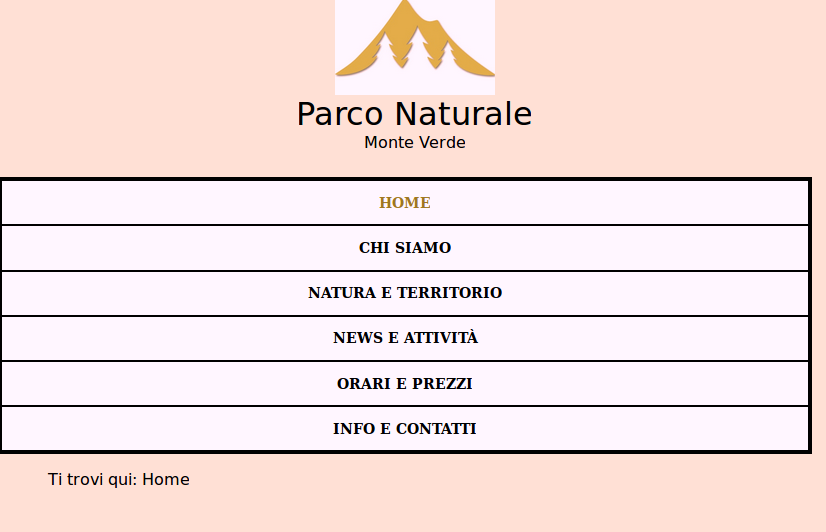
\includegraphics[width=90mm]{deuteranopia1}
			\caption{vedi file deuteranopia1.png}
			\end{figure} 

			\begin{figure}
			\centering
			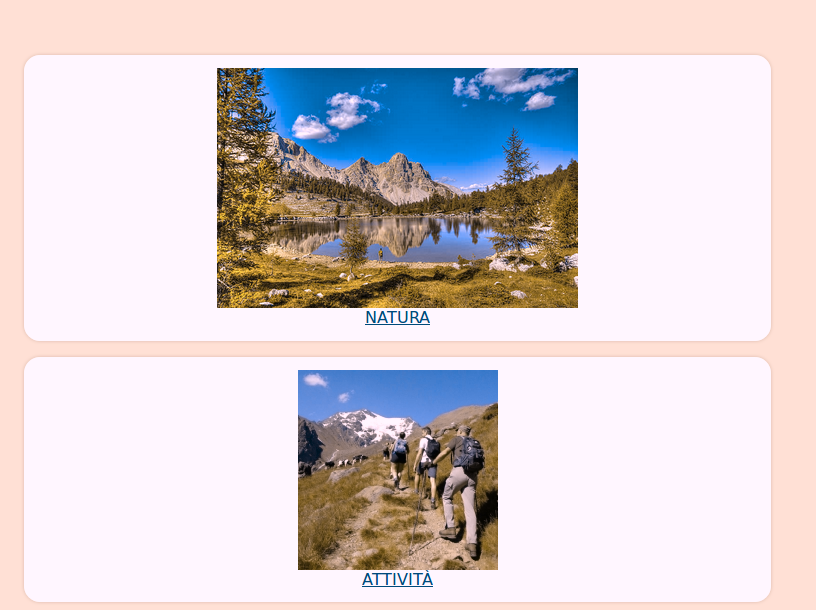
\includegraphics[width=90mm]{deuteranopia2}
			\caption{vedi file deuteranopia2.png}
			\end{figure}

			\begin{figure}
			\centering
			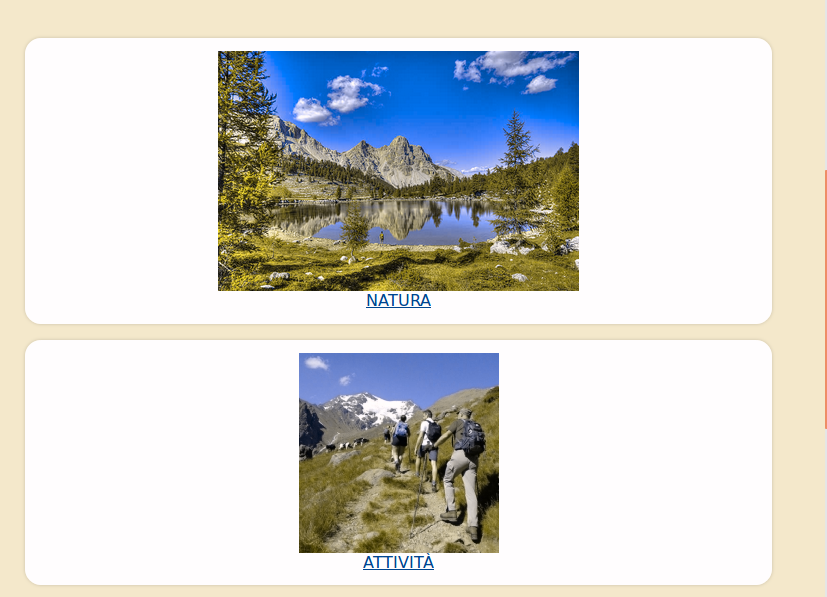
\includegraphics[width=90mm]{protanopia1}
			\caption{vedi file protanopia1.png}
			\end{figure}


			\begin{figure}
			\centering
			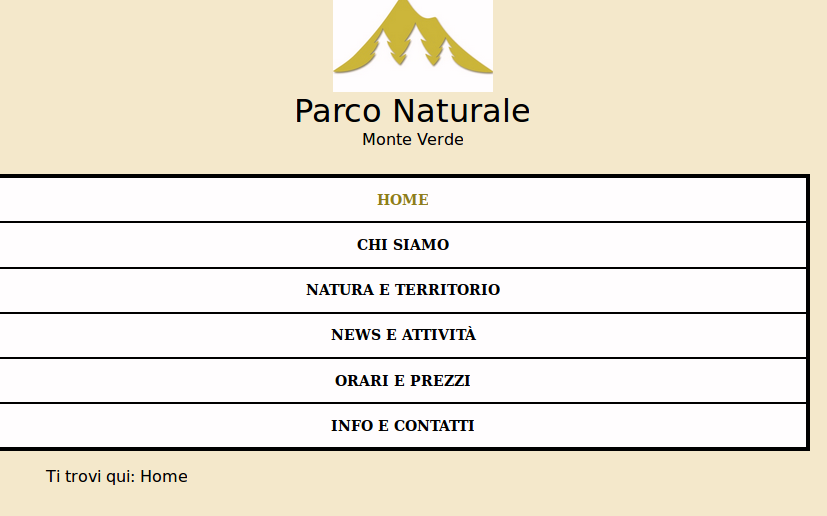
\includegraphics[width=90mm]{protanopia2}
			\caption{vedi file protanopia2.png}
			\end{figure}


			\begin{figure}
			\centering
			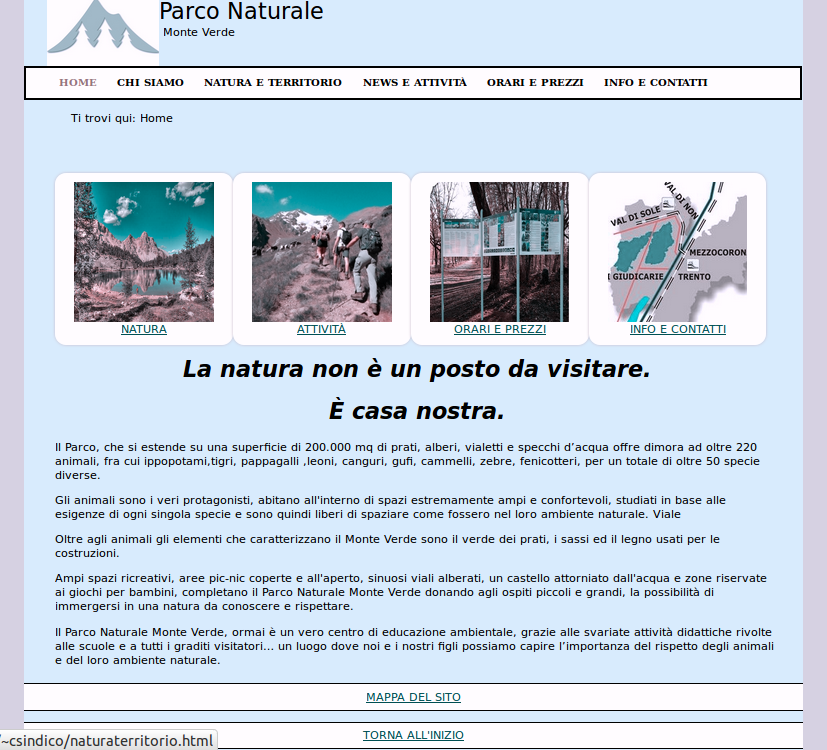
\includegraphics[width=90mm]{tritanopia1}
			\caption{vedi file tritanopia1.png}
			\end{figure}
			
			\begin{figure}
			\centering
			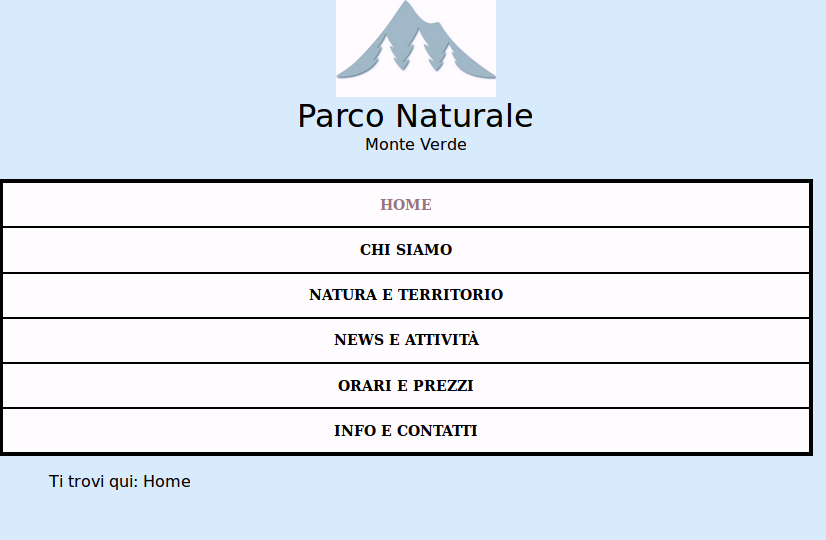
\includegraphics[width=90mm]{tritanopia2}
			\caption{vedi file tritanopia2.png}
			\end{figure}
						
			\item Sono stati inseriti per ogni pagina i tag meta:
	 		\begin{itemize}
				\item title: descrive la pagina corrente dal particolare al generale.
				\item description: da una descrizione del contenuto del sito
				\item keywords: contiene parole chiave per i motori di ricerca
				\item language: indica che il sito \'e stato interamente scritto in italiano.
				\item author: indica l'autore/i del sito
				\item content-type: contiene direttive per il browser (in particolare per l'utilizzo degli script Javascript)
				\item viewport: esprime indicazioni per la visualizzazione
			\end{itemize}
		
				\item Ogni foto ha il suo attributo alt che descrive ci\'o che l'immagine ritrae.
				Si \`e evitato di utilizzare immagini per visualizzare il testo, quindi il contenuto informativo rimane accessibile anche quando fallisce il caricamento delle immagini o del CSS.
				\item Si \'e prestata particolare attenzione alle parole straniere che sono state segnalate agli screenreader attraverso il tag "span xml:lang=en" segnalando la lingua con cui leggere correttamente i vocaboli. 
				\item In tutte le pagine, \`e stato inserito un link \textit{skip-nav} per saltare direttamente al contenuto qualora l'utente dello screen reader non voglia riascoltare nuovamente il men\`u
				\item Non sono state utilizzate tabelle per la gestione del layout grafico
				\item Non sono presenti oggetti java o flash non accessibili
				\item Nei form si \`e cercato di associare in maniera esplicita le etichette ai rispettivi controlli, posizionandole in modo che sia agevolata la compilazione dei campi da parte di chi utilizza tecnologie assistive
				\item Tutti gli elementi informativi e le funzionalit\`a sono disponibili anche in assenza del colore utilizzato per presentarli nelle pagine
				\item Il contrasto tra lo sfondo e il contenuto informativo è garantito da un sufficiente contrasto
				\item Non sono presenti oggetti e scritte lampeggianti o in movimento le cui frequenze di intermittenza possano provocare disturbi di epilessia fotosensibile o disturbi della concentrazione ovvero possano causare il malfunzionamento di tecnologie assistive utilizzate dall’utente
				\end{itemize}
	
	
\end{document}
